\documentclass{article}

% Language setting
% Replace `english' with e.g. `spanish' to change the document language
\usepackage[english]{babel}

% Set page size and margins
% Replace `letterpaper' with `a4paper' for UK/EU standard size
\usepackage[a4paper,top=2cm,bottom=2cm,left=3cm,right=3cm,marginparwidth=1.75cm]{geometry}

% Useful packages
\usepackage{caption}
\usepackage{amsmath}
\usepackage{graphicx}
\usepackage[colorlinks=true, allcolors=blue]{hyperref}

\usepackage{tikz}
% Node styles
\tikzstyle{dot}=[fill={rgb,255: red,175; green,237; blue,255}, draw=black, shape=circle]
\tikzstyle{mote}=[fill={rgb,255: red,255; green,128; blue,130}, draw=black, shape=rectangle]
% Edge styles
\tikzstyle{ed}=[-, draw=black]


\title{IoT Optional Project - Hidden Terminal}
\author{\Large Marco Somaschini 10561636} 
\date{
	\small
	\parbox{\linewidth}{
	\centering
  		Prof. Matteo Cesana
	\endgraf\smallskip
 		 Academic Year 2021/2022
}}

\begin{document}
\maketitle
\newpage

\tableofcontents
\newpage

\section{Introduction}
The hidden terminal is one of the classical problems of wireless communication. A typical scenario is that of multiple different terminals trying to communicate with the same node, which acts as a base station for operations. The base station falls in the transmission range of all these terminals (and vice versa), but the same isn’t always true between a terminal and the others. If two or more terminals can’t communicate directly, then it’s impossible for them to implement any multiple access communication protocol, like ALOHA or CSMA/CA, and collisions will likely occur as they try to simultaneously transmit to the station. This project aims at simulating this scenario and illustrating how the hidden terminal problem can be solved through the introduction of the RTS/CTS protocol.

\subsection{Tools Used}
The project was realized using TinyOS framework to code the network’s behaviour and TOSSIM python library for simulating it. The starting point was the template application proposed during the course challenge on TOSSIM, which was modified accordingly. The whole project has been uploaded on \href{https://github.com/MarcoSomaschini/iot-hidden-terminal-TOSSIM/tree/rts-cts}{Github}. The git repo contains two different branches: master and rts-cts. The first branch hosts a version of the application that do not implement the RTS/CTS protocol, while the second branch hosts one that does. In this way it’s possible to compare the network behaviour in both situations.

\subsection{Assumptions}
\begin{itemize}
  \item The motes were assumed to produce packets according to a Poisson distribution with a specific lambda. 
  \item The network was assumed to be composed by six motes: one base station and five terminals. Furthermore, three motes were arranged to create a subnet together with the base station, while the other two were isolated. As a consequence, these two isolated motes would result hidden to each other and to the other three.
  
  \begin{center}
      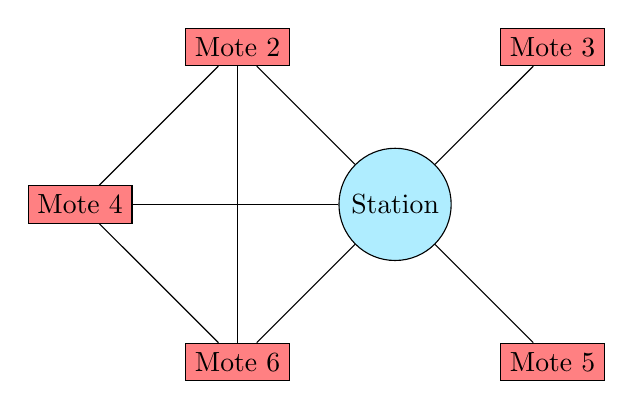
\begin{tikzpicture}
    	\node [style=mote] (0) at (-4, 0) {Mote 4};
    	\node [style=mote] (1) at (2, -2) {Mote 5};
    	\node [style=mote] (2) at (-2, 2) {Mote 2};
    	\node [style=mote] (3) at (-2, -2) {Mote 6};
    	\node [style=mote] (4) at (2, 2) {Mote 3};
    	\node [style=dot] (5) at (0, 0) {Station};
    	\draw (5) to (2);
    	\draw (0) to (2);
    	\draw (0) to (3);
    	\draw (3) to (5);
    	\draw (5) to (0);
    	\draw (2) to (3);
    	\draw (4) to (5);
    	\draw (1) to (5);
    \end{tikzpicture}
    \captionof{figure}{Network Topology}
  \end{center}
  
  \item The motes forming the subnet were assumed to implement a simple CSMA protocol to avoid collisions between them. This is needed because, without implementing any communication protocol, these motes would act just like they were hidden from one another.
\end{itemize}

\newpage

\section{Implementation}
\subsection{Poisson Distribution}
The Poisson distribution was generated indirectly, by computing the inter-arrival time between each packet generation. The time interval between events of a Poisson process can be modelled as an exponential distribution $E(\lambda)$. To simulate such a distribution the \textit{RandomC} component was used to extract a random 16-bit number and then mapping it to a value in $[0, 1]$, thus obtaining a sample from a uniform distribution. Then, leveraging the inverse cumulative distribution function for an exponential distribution $E(\lambda)$, the inter-arrival time was computed as: $F^{-1}(p, \lambda) = -\frac{\log{1- p}}{\lambda}$. After booting, each mote generated a time interval according to its $\lambda$ and set a timer of such length. The firing of the timer was interpreted as the arrival of a new packet. After the handling of the packet a new interval was computed, and a new timer set.

\subsection{Baseline Communication Protocol}
The baseline mote-station exchange worked as such: whenever a packet was ready, the mote would send it to the base station and wait for an ACK. This was done using the \textit{AMSenderC} and \textit{AMReceiverC} components. If a packet wasn’t acked, the mote would simply retry sending it. The packets contained a sequence number and a field indicating how many times their transmission had been attempted. The base station, upon receiving a packet, would do some computation on it before replying with an ACK and logging its sequence number and total attempted transmissions, in order to compute the relative mote PER. The packet computation was simulated using the \textit{FakeSensorC} component, that simply stalled for a short amount of time through a timer. This was needed as otherwise the entire exchange would be way too fast and unrealistic.

\subsection{CSMA protocol}
The CSMA protocol implemented by the three subnet motes consisted in sensing the channel before starting a transmission and backing-off if an undergoing communication was detected. The channel sensing was simulated using a global variable, which the subnet motes (only them) would check before attempting any transmissions. If the variable evaluated as FALSE, then the mote sensing it would set it to TRUE and start transmitting to the base station. Any subsequent mote would then detect that the channel was busy and back-off for a random amount of backoff periods randomly picked in $[0, 2^{BE} - 1]$. After receiving an ACK for the packet sent, the transmitting mote would set the sensing variable back to FALSE and thus free the channel.

\subsection{RTS/CTS}
The RTS/CTS version was built on top of the previous functionalities. In this version, before sending a packet, a mote sent an RTS message in broadcast and then stalled, waiting for a CTS from the base station. Upon receiving an RTS, any terminal mote was made to stall for a given amount of time. The base station, instead, would reply by sending a CTS message in broadcast and then wait for a packet. Again, any mote would stall for a given time upon receiving a CTS message, except for the terminal that requested it. Such mote would then proceed by sending the generated packet to the base station. The stalling was implement through the use of a timer and a Boolean variable, indicating if the mote was allowed to send.

\subsection{Logging}
The base station also kept track of the total elapsed time of the simulation, in order to stop accepting packets after a certain period. While ending the simulation, the base station printed the motes transmission stats, useful to understand the effectiveness of the protocols.

\newpage

\section{Conclusions}
The simulations where set to account for five minutes of network activity and the following results were gathered.

\subsection{No RTS/CTS}
The first version, that didn't implement RTS/CTS, saw very high PERs, in the order of 10\%. It can be noticed that the motes falling in the CSMA subnet have a slightly (around 1\%) lower PER, due to collisions only happening with outsider motes. The average transmission rates approach the motes' $\lambda$ as expected.

\begin{center}
  \includegraphics[width=8cm]{images/NO_RCTS.jpg}
  \captionof{figure}{No RTS/CTS motes transmissions stats}
\end{center}

\subsection{RTS/CTS (250ms of wait time)}
The version implementing RTS/CTS, instead, showed much lower PERs, around 3-5\%. Indeed, the introduction of the protocol managed to avoid a significant number of collisions. It must be said that the average average transmission rates of the motes decreased significantly, due to the overhead and extra synchronization effort required.

\begin{center}
  \includegraphics[width=8cm]{images/RCTS.jpg}
  \captionof{figure}{RTS/CTS motes transmissions stats}
\end{center}

\subsection{RTS/CTS (100ms of wait time)}
Running a simulation using the same version as before but with a significantly shorter wait time, which is the fixed amount of time nodes stops after receiving an RTS/CTS, it can be seen that the PERs increase by a couple percentage points but the average transmission rates increase as well. In conclusion, the wait time seems to be a parameter that controls the PER/throughput trade-off.

\begin{center}
  \includegraphics[width=8cm]{images/RCTS_100.jpg}
  \captionof{figure}{RTS/CTS motes transmissions stats with shorter wait time}
\end{center}


\end{document}